\chapter{General Description of the User Interface} \label{cha:interface}
\section{The user interface components}
QDOAS is based on the notion of \textit{projects}. A project is as a set of files sharing
the same configuration of analysis, i.e. the definition of spectral windows and the list of files to be analysed with this configuration.

QDOAS allows defining several projects in a session, giving users the possibility to handle several analysis configurations.

\begin{center}
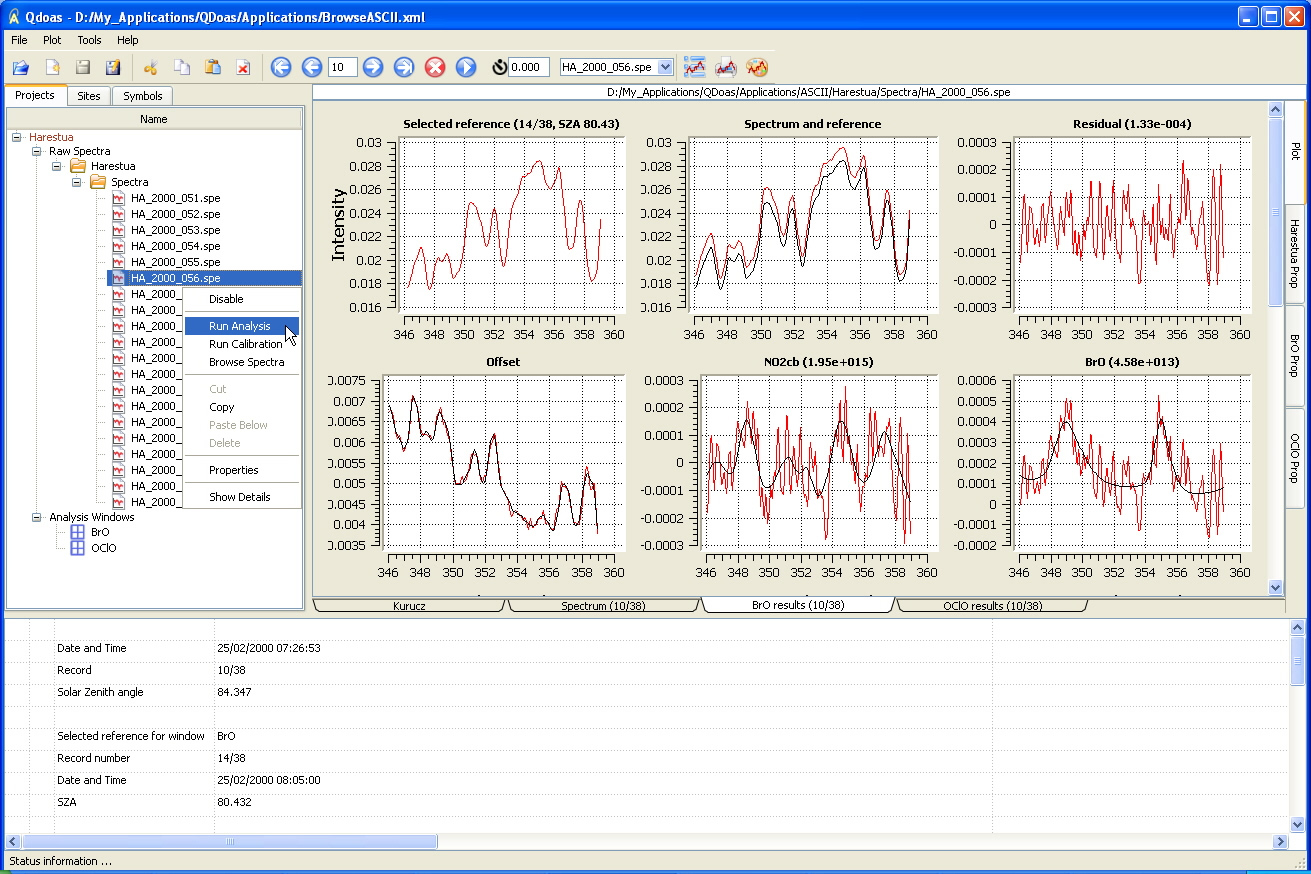
\includegraphics[width=1\textwidth,angle=0]{img/QDOAS_UI.jpg}
\end{center}

QDOAS user interface and configuration property sheets are distributed into three resizable panels with a fixed
arrangement~:

\begin{qdoasitem}
\item the elements of the application organized in tree structures
  presented in three tab pages (\textbf{Projects}, \textbf{Sites} and \textbf{Symbols}) in the
  upper-left one;
\item dialog boxes for the configuration of the elements of the
  application and the plot of spectra and results in the upper-right
  one; all the spectral windows are processed in one shot; right and
  bottom tab- switched access possible between all these pages;
\item the available information on the current spectrum and analysis
  results are displayed in the third one;
\end{qdoasitem}

\subsection{The Menu Bar}\hfill
\begin{minipage}[t]{\textwidth}
\vspace{-0.6\baselineskip}
\begin{tabular}[h]{p{2cm} p{9.5cm}}
\textbf{File} & Usual option to create a new application, open an existing
  one or save the current settings. QDOAS configuration files are in
  XML format.  \\ [6pt]
\textbf{Plot} & New option to organize the plots on the page (see below),
  to print the plot page or to save it in a png file; \\ [6pt]
\textbf{Tools} & The Convolution, Ring and undersampling tools are modules completely independent from the
  QDOAS application but they can still be called from the user
  interface;  \\ [6pt]
\textbf{Help} & Access to on-line help
\end{tabular}
\end{minipage}

\subsection{The Toolbar} \label{sec:interface_toolbar}
\hfill\vspace{-.8\baselineskip}
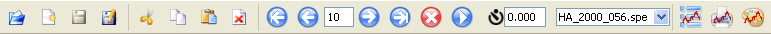
\includegraphics[width=\textwidth]{img/QDOAS_Toolbar.jpg}
The toolbar gives access to the same \textbf{File} and \textbf{Plot}
options of the menu bar. It contains also buttons to move easily in
the current file or to use another file in the case a multiple files
selection has been performed (very useful to browse spectra in the \textbf{MFC format (binary or std) generated by DOASIS} (cfr page \pageref{sec:MFC_DOASIS})).

\begin{minipage}{\textwidth} %minipage to force title and image to be on the same page
\subsection{Plot Properties}
\hfill\vspace{-.8\baselineskip}
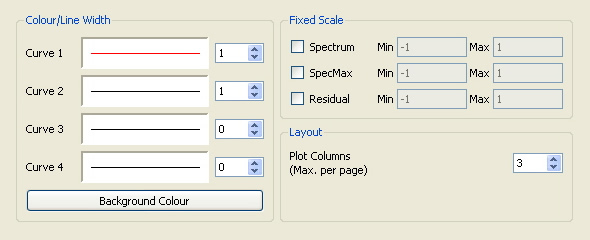
\includegraphics[width=\textwidth]{img/Plot_Properties.jpg}
This dialog box allows selecting a different color and a different
line thickness for curves 1 and 2 (respectively the spectrum and the
reference or the observed optical depth and the calculated optical
depth). The number of plot columns impacts the size of the plots.
\end{minipage}

\subsection{Handling plots}
It is not possible to display a specific plot in another window but zoom can be made by right-clicking the
\textbf{Interactive} option from \underline{\textbf{the title of a plot}}.

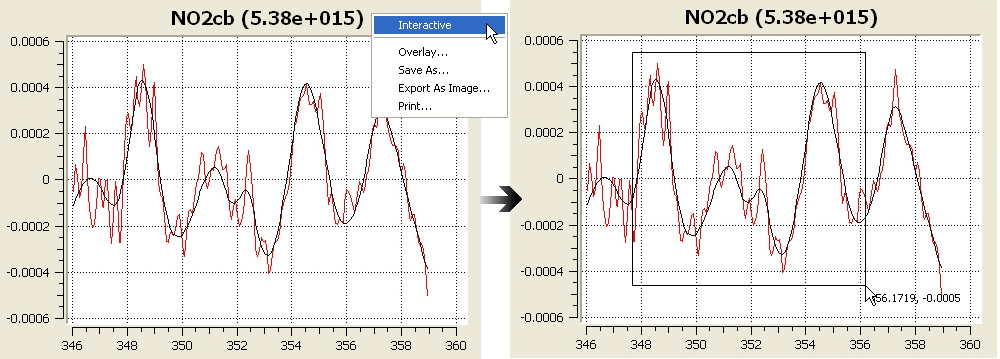
\includegraphics[width=\textwidth]{img/Plot_Zoom.jpg}

The \textbf{Save As} option saves the plotted curves in a ASCII file
(useful for example to create a reference spectrum). \textbf{Export As}
image exports the selected plot in a png file while \textbf{Print}
sends it to printer. \textbf{Overlay} will load a spectrum from a given file
and superpose it over the already plotted curves but this option is
not yet implemented.

\section{The projects tree}
The organisation of projects, analysis windows, spectra files and
directories in a tree structure completed with the definition of
right-click shortcut menus at each level of the tree makes the access,
manipulation and con\-fi\-gu\-ra\-tion of all these objects very easy.

\subsection{Raw Spectra}
Spectra to analyze have to be inserted under this projects tree
node. Individual files and complete directories structures are
accepted. The ``New Folder" option allows organizing spectra files and
directories within a user-defined catalog (folder that is not
physically present on the disk). The following actions can be
performed from any node:

\begin{tabular}[h]{p{3.5cm} p{8cm}}
\textbf{Browse Spectra} & browses spectra in the selected file(s); \\ [6pt]
\textbf{Run Analysis} & analyses spectra using the configuration
  of the project and analysis windows; this step includes the
  correction of the wavelength calibration of the reference spectrum
  if it has been requested in the configuration of the analysis
  windows; \\ [6pt]
\textbf{Run Calibration} & uses the options defined in the
  \textbf{Calibration page} of \textbf{Projects properties} (see page \pageref{sec:projects_calibration_page}) to apply it on
  spectra. \\ [6pt]
\textbf{Export Data/Spectra} & browses spectra and saves the selected fields in ASCII .  If only data on records are exported, the format is the same as QDOAS \textbf{output} files (see Annex, page \pageref{cha:output}); otherwise, spectra are saved in \textbf{Column extended format} (see Annex, page \pageref{cha:input-files-format}) \\ [6pt]
\end{tabular}

To move from one record to the other or from one file to the other (in
case of multiple files selection), use the adequate buttons in the
toolbar:

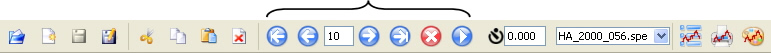
\includegraphics[width=\textwidth]{img/QDOAS_Toolbar2.jpg}

Other options~:

\begin{tabular}[h]{p{4cm} p{7.5cm}}
\textbf{Disable/Enable} & Disables the selected file or directory
  from the list of files to browse/analyze. Enable option re-enables
  previously disabled files. \\ [6pt]
\textbf{Refresh} & Refreshes the list of files in the selected
  directory;    \\ [6pt]
\textbf{Show/Hide Details} & Shows/hides file information (last
  modification date and time, size). The file size information is
  useful to indicate if the selected file is empty or not. \\ [6pt]
\end{tabular}


\subsection{Analysis windows}
A project can include several spectral analysis windows. A specific
analysis window can be disabled in order not to process it without
removing it from the list. The \textbf{View Cross Sections} option is
useful to check that the requested cross sections files exist.

\section{The observation sites}
In the \textbf{Observation Sites} page, a list of observation sites
can be specified by their location coordinates:

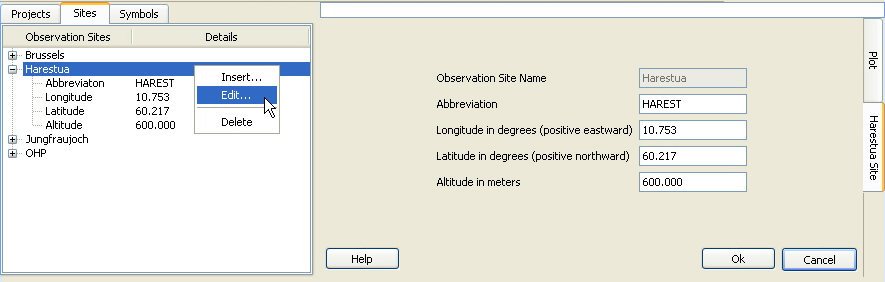
\includegraphics[width=\textwidth]{img/Observation_Sites.jpg}

QDOAS applies the following conventions~:

\begin{minipage}[t]{\textwidth}
\vspace{-1\baselineskip}
\begin{itemize} \itemsep -6pt
\item longitudes are positive eastwards; negative westwards;
\item latitudes are positive northwards; negative southwards.
\end{itemize}
\end{minipage}

For ground-based measurements, information on the observation site can
help to [re-]calculate the solar zenith angle as far as the
measurement date and time are correct (see the \textbf{Instrumental page}
 of \textbf{Projects properties}, page \pageref{sec:projects_instrumental_page}).
The longitude is also accounted to correctly select the reference spectrum of the day using the local time instead of the UT time in the case fractional days and times given in UT are distributed on two days (for example, for China data, two reference spectra could be selected for data of a same day before and after 00:00 UT if the observation site is not specified).

 For satellite
measurements, this page can be used to define a list of overpasses
(see the \textbf{Selection} page of Projects properties, page \pageref{sec:projects_selection_page}). In
both cases, the \textbf{Abbreviation} is used as prefix of the name of
the output files when the automatic creation of the output file name
is requested.

The \textbf{Altitude} information is just for the user.

\section{The symbols}
Before configuring the analysis, the user must define the list of all
relevant symbols that will be used. These symbols are needed to build
cross sections files filters, to link \gls{amf} and cross section files and
for internal manipulations (\textbf{Molecules} and \textbf{Shift and
  Stretch} pages of \textbf{Analysis Windows properties}).

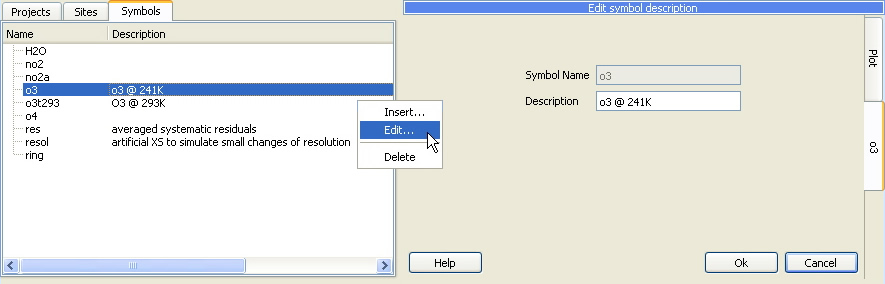
\includegraphics[width=\textwidth]{img/Symbols.jpg}

Cross sections symbols can be completed with a short description. The
deletion of a symbol is possible only if this symbol is not used in
the configuration of a project or an analysis window.

%%% Local Variables:
%%% mode: latex
%%% TeX-master: "QDOAS_manual"
%%% TeX-PDF-mode: t
%%% End:
